\documentclass[conference,a4paper]{IEEEtran}
\IEEEoverridecommandlockouts

\usepackage[utf8]{inputenc}
\usepackage[T1]{fontenc}
\usepackage[spanish,es-tabla,es-noshorthands,es-nolists]{babel}
\usepackage{cite}
\usepackage{amsmath}
\usepackage{newtxtext,newtxmath}
\usepackage{graphicx}
\usepackage{booktabs}
\usepackage{multirow}
\usepackage[locale=FR,group-digits=integer,group-minimum-digits=4,group-separator={.}]{siunitx}
\usepackage{xurl}
\usepackage{xcolor}

\graphicspath{{../figures/}{figuras/}}
\sisetup{detect-all}

\begin{document}

\title{Detección temprana de incendios con YOLO11:\\
detector, clasificador de recortes y criterio temporal sobre D-Fire}

\author{
\IEEEauthorblockN{Martín Amagliani, Tatiana Durán, Tomás Frechou}
\IEEEauthorblockA{Carrera de Especialización en Inteligencia Artificial (CEIA)\\
Facultad de Ingeniería, Universidad de Buenos Aires\\
Visión por Computadora II -- Equipo 7}
}

\maketitle

\begin{abstract}
Presentamos un prototipo de alerta temprana de incendios a partir de video que combina tres etapas: un detector YOLO11 de fuego y humo ajustado sobre D-Fire, un clasificador liviano que confirma o descarta cada recorte detectado y un criterio temporal K-de-N con estados normal, prealerta y alerta. Comparamos cuatro configuraciones del detector variando capacidad, resolución de entrada y presencia de imágenes negativas en el entrenamiento, y medimos latencia en CPU. El modelo \textit{nano} a \SI{640}{px} alcanza un mAP50 de \num{0.759} en test con \SI{56}{ms} por frame en CPU; el modelo \textit{medium} gana solo \num{0.020} de mAP50 a un costo cinco veces mayor. Entrenar con imágenes negativas reduce las imágenes sin incendio con algún falso positivo de \SI{28.8}{\percent} a \SI{0.65}{\percent} sin perder recall, y el clasificador de recortes las lleva a \SI{0.10}{\percent} a cambio de \num{4.5} puntos de recall en humo. Además, mostramos que cerca de la mitad de las imágenes del test oficial de D-Fire tienen un casi-duplicado en entrenamiento, por lo que las métricas sobre ese split son optimistas.
\end{abstract}

\begin{IEEEkeywords}
detección de incendios, detección de humo, YOLO11, D-Fire, falsos positivos, criterio temporal
\end{IEEEkeywords}

% ---------------------------------------------------------------------------
\section{Introducción}

Un incendio forestal detectado en sus primeros minutos puede contenerse con pocos recursos; detectado tarde, puede volverse incontrolable. Las redes de cámaras fijas en cerros y torres son una forma barata de vigilar grandes superficies, pero mirarlas en forma continua es inviable para operadores humanos. Por eso la detección automática de humo y fuego con visión por computadora se volvió un área activa \cite{jin2023videofire}.

El caso real más visible es el de California. Desde 2023, CAL FIRE y el programa ALERTCalifornia de la Universidad de California San Diego operan un sistema de IA desarrollado junto con DigitalPath que analiza más de \num{1000} cámaras y avisa a los centros de despacho cuando detecta una anomalía compatible con humo. El piloto comenzó en seis centros de comando y en septiembre de 2023 se extendió a los 21 centros de despacho del estado \cite{alertca2023time}. En uno de los primeros casos, el sistema alertó un incendio iniciado a las 3 de la mañana en el Bosque Nacional Cleveland, que fue extinguido en 45 minutos \cite{reuters2023california}. Dos rasgos de ese sistema guían nuestro diseño: las alertas son verificadas por operadores, porque nubes, niebla y polvo generan falsos positivos, y lo que importa operativamente no es el mAP de cada imagen sino cuántas falsas alarmas por hora recibe un operador y cuánto tarda en llegar una alerta verdadera.

En Argentina, tras el incendio de El Bolsón de 2025, que afectó 221 viviendas, el Servicio de Prevención y Lucha contra Incendios Forestales (SPLIF) de Río Negro incorporó Aleph-fuego, una plataforma desarrollada por INVAP que reconoce columnas de humo en cámaras con cobertura de \ang{360} y envía alertas al centro de monitoreo. El sistema opera en Bariloche y El Bolsón y se está extendiendo a otras localidades de la provincia \cite{rionegro_splif_ia,diarioneuquino2026aleph}.

El objetivo de este trabajo es construir y evaluar un prototipo que, a partir de un flujo de video, emita alertas de fuego o humo con pocas falsas alarmas y latencia compatible con CPU. Nuestras contribuciones son:
\begin{itemize}
\item Un sistema de tres etapas (detector, clasificador de recortes y criterio temporal K-de-N) con código reproducible y una demo que procesa video en tiempo real.
\item Un estudio controlado del detector que aísla el efecto de la capacidad del modelo, la resolución de entrada y las imágenes negativas, con métricas por clase y latencia en CPU y GPU.
\item Evidencia cuantitativa de fuga entre los splits oficiales de D-Fire mediante \textit{hashing} perceptual, y sus implicancias para interpretar las métricas.
\end{itemize}

% ---------------------------------------------------------------------------
\section{Trabajos relacionados}

D-Fire \cite{venancio2022dfire} es un conjunto de más de \num{21000} imágenes anotadas con cajas de fuego y humo, con una fracción grande de imágenes negativas. Sus autores entrenaron detectores YOLOv4 y aplicaron poda de filtros para ejecutarlos en una Raspberry Pi 4, reduciendo el costo computacional hasta un \SI{83.6}{\percent}. FIgLib y SmokeyNet \cite{dewangan2022figlib} abordan el problema desde cámaras fijas de la red HPWREN: FIgLib reúne cerca de \num{25000} imágenes etiquetadas de secuencias alrededor de cada ignición, y SmokeyNet explota la información espaciotemporal de varias imágenes consecutivas, con desempeño comparable al humano. Nuestro criterio temporal persigue el mismo objetivo con una regla determinística sobre las detecciones, sin un modelo temporal adicional.

Elegimos detectores de una etapa de la familia YOLO \cite{redmon2016yolo} en lugar de detectores de dos etapas como Faster R-CNN \cite{ren2015faster} porque el sistema debe procesar varios frames por segundo en CPU. Usamos YOLO11 \cite{khanam2024yolo11,ultralytics2024yolo11}, preentrenado en COCO \cite{lin2014coco}, que ofrece variantes de distinta capacidad (\textit{nano} a \textit{x-large}) con la misma API para detección y clasificación.

% ---------------------------------------------------------------------------
\section{Dataset y análisis exploratorio}

Usamos la distribución de D-Fire en formato YOLO con su split oficial: \num{14122} imágenes de entrenamiento, \num{3099} de validación y \num{4306} de prueba, con dos clases (\textit{smoke} y \textit{fire}). El \SI{45.7}{\percent} de las imágenes son negativas, sin fuego ni humo (entre \SI{44.4}{\percent} y \SI{46.6}{\percent} según el split), y en total hay \num{14685} cajas de fuego y \num{11854} de humo.

\textbf{Fuego chico, humo grande.} Las dos clases tienen escalas muy distintas. La mediana del área relativa de una caja es \num{0.0054} para fuego y \num{0.142} para humo. Tras el \textit{letterbox} a \SI{640}{px}, el \SI{45.0}{\percent} de las cajas de fuego es \textit{small} según el criterio de COCO (área menor a $32^2$ px), contra el \SI{12.2}{\percent} de las de humo; la mediana del lado es \SI{36}{px} para fuego y \SI{186}{px} para humo. A \SI{960}{px} la fracción de fuego \textit{small} baja al \SI{27.7}{\percent}. Esto motiva la hipótesis H1 sobre resolución.

\textbf{Fuga entre splits.} D-Fire incluye frames extraídos de videos y de cámaras fijas, por lo que dos imágenes pueden ser la misma escena sin ser idénticas byte a byte. No hay duplicados exactos (MD5) entre splits, pero al comparar un \textit{difference hash} de 64 bits de cada imagen de prueba contra todo el entrenamiento, el \SI{21.8}{\percent} tiene una imagen a distancia de Hamming 0 y el \SI{49.9}{\percent} a distancia $\le 4$, que en la práctica es la misma escena. La fuga afecta tanto a negativas (\SI{61.1}{\percent} a distancia $\le 4$) como a imágenes con solo fuego (\SI{57.7}{\percent}) o solo humo (\SI{48.6}{\percent}). Mantenemos el split oficial para que los resultados sean comparables con la literatura, pero las métricas sobre él deben leerse como una cota optimista del desempeño en una cámara nueva.

% ---------------------------------------------------------------------------
\section{Metodología}

\begin{figure}[t]
\centering
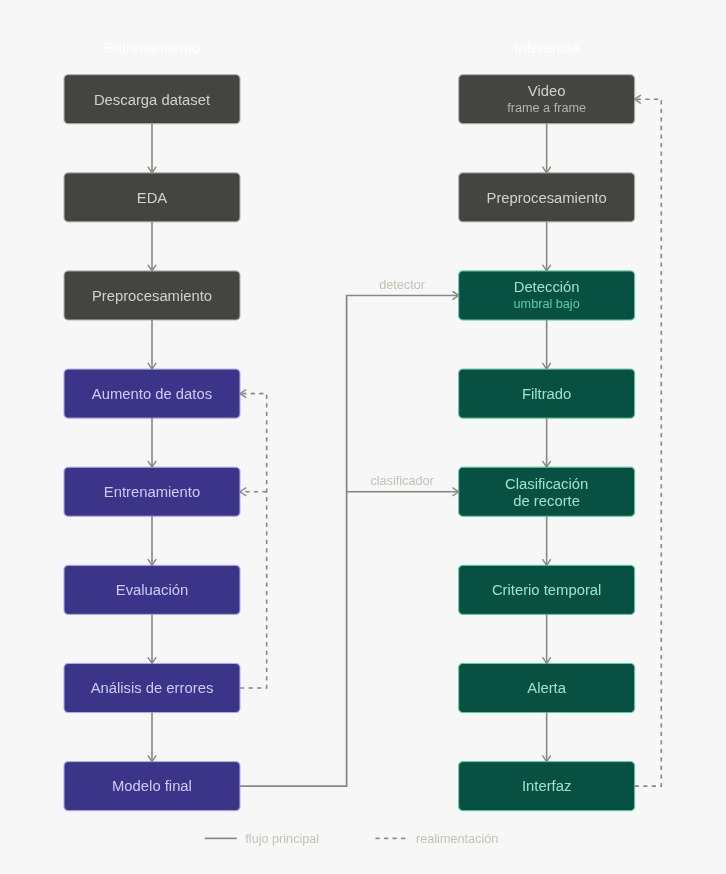
\includegraphics[width=0.78\columnwidth]{pipeline.jpg}
\caption{Pipeline del sistema. Izquierda: entrenamiento; derecha: inferencia sobre video. Las líneas punteadas indican realimentación.}
\label{fig:pipeline}
\end{figure}

La Fig.~\ref{fig:pipeline} resume el sistema. En inferencia, cada frame pasa por cuatro pasos.

\textbf{Detector.} YOLO11 ajustado sobre D-Fire, con cabeza de dos clases. Entrenamos 50 épocas con batch 16, semilla 42 y el aumento de datos por defecto de Ultralytics (mosaic, variación HSV, volteo horizontal y escalado), aplicado solo en entrenamiento. En inferencia usamos un umbral bajo ($\mathit{conf}_{\min}=0{,}05$) para no descartar candidatos, NMS, y un umbral operativo $\tau$ que decide qué detecciones cuentan para la alerta.

\textbf{Clasificador de recortes.} Cada caja con confianza mayor que $\tau$ se recorta con un margen de contexto del \SI{10}{\percent} por lado y se clasifica con un \texttt{yolo11n-cls} a \SI{224}{px} en \textit{real} o \textit{confundible}. Su dataset se construye solo con imágenes de entrenamiento: los positivos son cajas anotadas y los negativos son falsos positivos del detector sin negativas (R5, ver abajo) sobre las \num{6458} imágenes negativas de entrenamiento. Usamos R5 para minar porque, al no haber visto esas imágenes, sus errores se parecen a los que el sistema cometería en escenas nuevas. Las clases se balancean y la validación se separa por imagen. Una detección se \emph{confirma} si además $p_{\mathrm{real}} \ge 0{,}5$.

\textbf{Criterio temporal K-de-N.} Para cada clase se mantiene un buffer de los últimos $N$ frames procesados. Si al menos $K$ tienen una detección confirmada, la clase pasa a \textsc{alerta} y se emite un evento; con entre 1 y $K-1$ está en \textsc{prealerta}. Con histéresis, la clase permanece en alerta hasta que el buffer queda vacío, de modo que un incendio con detecciones intermitentes produce un solo evento. El estado global es el peor de las clases.

\textbf{Interfaz.} La demo genera un video anotado con las cajas (punteadas si el clasificador las descarta), el estado, el contador K/N por clase, la latencia por frame y un registro de eventos (Fig.~\ref{fig:demo}).

\textbf{Diseño experimental.} Entrenamos cuatro detectores para responder hipótesis concretas: R1 (\textit{nano}, \SI{640}{px}, con negativas) como base; R3 (\textit{medium}, \SI{640}{px}) para el compromiso capacidad--latencia; R4 (\textit{nano}, \SI{960}{px}) para H1, \emph{aumentar la resolución mejora el recall de objetos chicos}; y R5 (\textit{nano}, \SI{640}{px}, sin las negativas de entrenamiento) para H2, \emph{entrenar con negativas reduce los falsos positivos sin perder recall}. H3 plantea que \emph{el criterio temporal reduce las falsas alarmas con una latencia de alerta acotada}, y H4 que \emph{el clasificador de recortes reduce los falsos positivos con una pérdida de recall acotada}.

Además del mAP de Ultralytics, evaluamos cada sistema a un punto de operación fijo ($\tau=0{,}4$): emparejamos predicciones y cajas anotadas de la misma clase con IoU $\ge 0{,}5$, de mayor a menor confianza, y reportamos precisión, recall y la fracción de las \num{2005} imágenes negativas de prueba con al menos un falso positivo, que es la métrica más cercana a una falsa alarma. La latencia se mide en CPU (Intel Core i7 de 13.ª generación, batch 1, 100 imágenes de calentamiento y 300 medidas) y en GPU (NVIDIA L4).

% ---------------------------------------------------------------------------
\section{Resultados experimentales}

\subsection{Capacidad, resolución y latencia}

\begin{table}[t]
\centering
\caption{Detectores en el split de prueba de D-Fire. Latencia por imagen: CPU con batch 1 (benchmark propio); GPU L4, tiempo de inferencia por imagen reportado por Ultralytics en la evaluación.}
\label{tab:runs}
\setlength{\tabcolsep}{3.2pt}
\begin{tabular}{@{}lcccccrr@{}}
\toprule
 & & \multicolumn{2}{c}{mAP50} & & & \multicolumn{2}{c}{ms/img} \\
\cmidrule(lr){3-4}\cmidrule(lr){7-8}
Run & Config. & humo & fuego & mAP50 & mAP50-95 & CPU & GPU \\
\midrule
R1 & n, 640, neg   & \num{0.820} & \num{0.698} & \num{0.759} & \num{0.434} & \num{56}  & \num{1.0} \\
R3 & m, 640, neg   & \num{0.838} & \num{0.719} & \textbf{\num{0.779}} & \textbf{\num{0.455}} & \num{299} & \num{5.9} \\
R4 & n, 960, neg   & \num{0.829} & \num{0.716} & \num{0.773} & \num{0.444} & \num{92}  & \num{2.6} \\
R5 & n, 640, sin neg & \num{0.727} & \num{0.670} & \num{0.699} & \num{0.402} & \num{55}  & \num{1.0} \\
\bottomrule
\end{tabular}
\end{table}

La Tabla~\ref{tab:runs} resume los cuatro detectores. El fuego es la clase difícil en todas las configuraciones (mAP50 entre \num{0.06} y \num{0.12} por debajo del humo), consistente con su menor tamaño. Pasar de \textit{nano} a \textit{medium} mejora el mAP50 en \num{0.020} pero multiplica por \num{5.3} la latencia en CPU (de \SI{56}{} a \SI{299}{ms}, es decir, de 18 a 3 FPS). Como el criterio temporal necesita varios frames por segundo y una latencia mayor retrasa la alerta, elegimos \textit{nano} como detector del sistema (Fig.~\ref{fig:tradeoff}).

\begin{figure}[t]
\centering
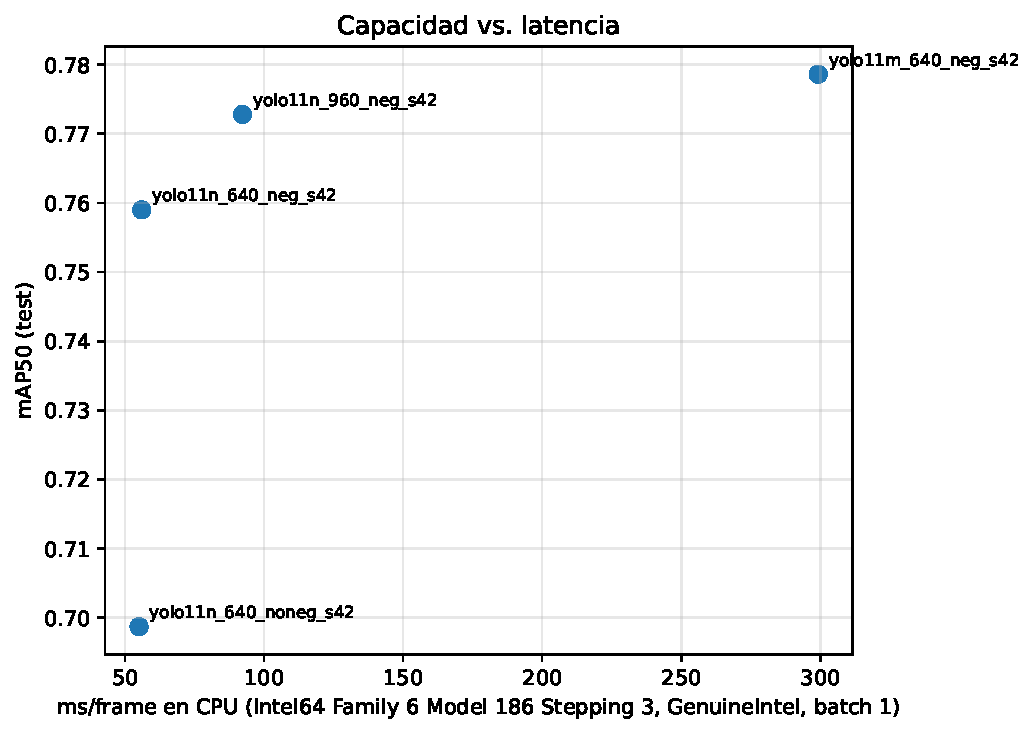
\includegraphics[width=0.82\columnwidth]{tradeoff_latencia}
\caption{Compromiso entre mAP50 en prueba y latencia en CPU (batch 1) de los cuatro detectores.}
\label{fig:tradeoff}
\end{figure}

\textbf{H1 (resolución).} R4 a \SI{960}{px} supera a R1 en \num{0.014} de mAP50 con \num{1.65} veces su latencia. La Tabla~\ref{tab:h1} muestra que la mejora se concentra en los objetos chicos: el recall de fuego \textit{small} sube \num{3.4} puntos y el de humo \textit{small} \num{4.6}, mientras que en objetos grandes no mejora (en fuego cae \num{2.6} puntos). H1 se confirma, pero el efecto es moderado: aun a \SI{960}{px}, menos de la mitad del fuego chico se detecta, por lo que la resolución por sí sola no resuelve la detección de focos incipientes.

\begin{table}[t]
\centering
\caption{H1: recall a $\tau=0{,}4$ por tamaño de caja (categorías COCO medidas a \SI{640}{px}) para R1 y R4.}
\label{tab:h1}
\begin{tabular}{@{}llrcc@{}}
\toprule
Clase & Tamaño & Cajas & R1 (640) & R4 (960) \\
\midrule
\multirow{3}{*}{fuego} & small  & \num{1318} & \num{0.405} & \textbf{\num{0.439}} \\
                       & medium & \num{1137} & \num{0.653} & \num{0.656} \\
                       & large  & \num{423}  & \textbf{\num{0.747}} & \num{0.721} \\
\midrule
\multirow{3}{*}{humo}  & small  & \num{302}  & \num{0.487} & \textbf{\num{0.533}} \\
                       & medium & \num{490}  & \num{0.618} & \num{0.637} \\
                       & large  & \num{1523} & \num{0.795} & \num{0.791} \\
\bottomrule
\end{tabular}
\end{table}

\subsection{Imágenes negativas (H2)}

\begin{figure}[t]
\centering
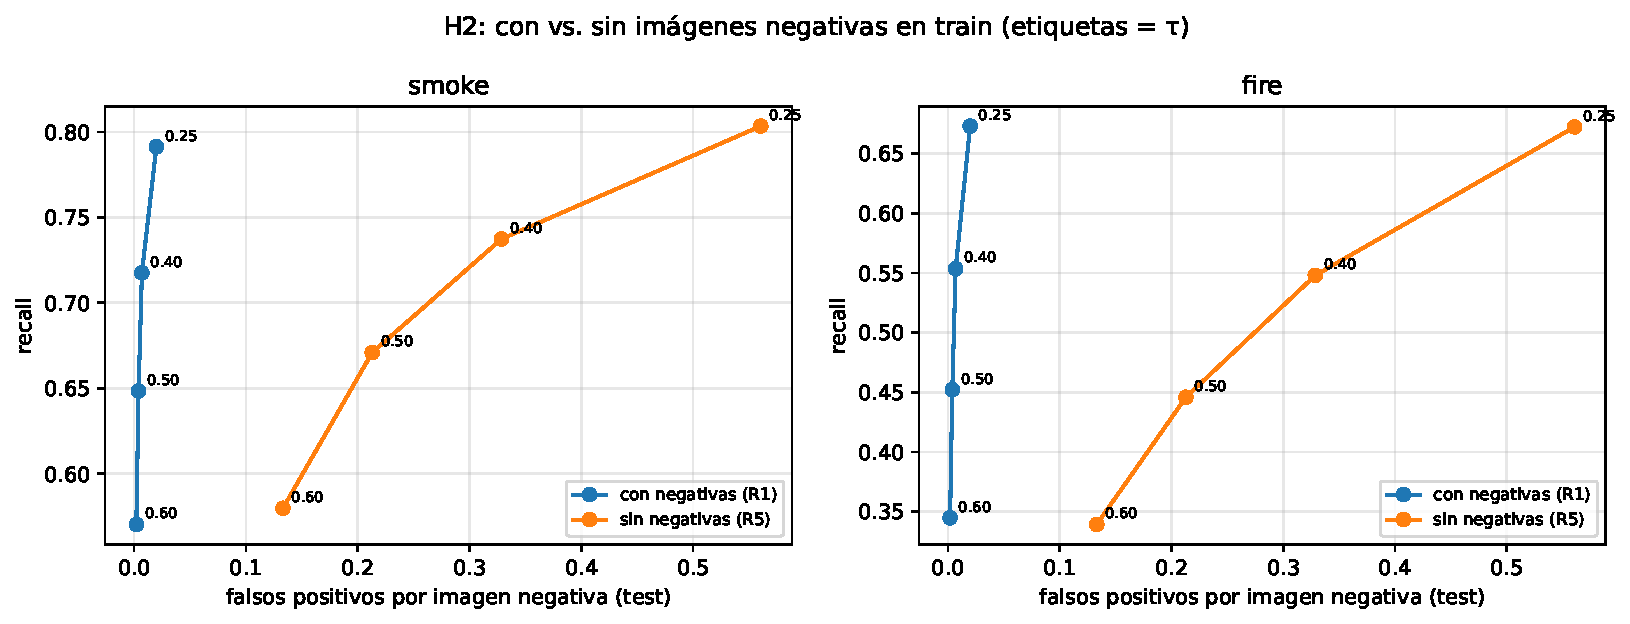
\includegraphics[width=\columnwidth]{h2_negativas}
\caption{H2: recall contra falsos positivos por imagen negativa de prueba al variar $\tau$, entrenando con (R1) y sin (R5) imágenes negativas.}
\label{fig:h2}
\end{figure}

Este es el efecto más fuerte del estudio. A $\tau=0{,}4$, sin negativas en entrenamiento (R5) el \SI{28.8}{\percent} de las imágenes negativas de prueba tiene al menos un falso positivo (\num{0.33} por imagen); con negativas (R1) la cifra baja a \SI{0.65}{\percent} (\num{0.007} por imagen), una reducción de 44 veces. El recall prácticamente no cambia (humo \num{0.717} contra \num{0.737}, fuego \num{0.554} contra \num{0.548}) y la precisión en humo sube de \num{0.663} a \num{0.846}. La Fig.~\ref{fig:h2} muestra que la curva de R1 domina a la de R5 en todo el rango de $\tau$: no hay un umbral al que R5 iguale a R1, de modo que la diferencia no es una cuestión de calibración. H2 se confirma. Hay que tener en cuenta que parte de esta ventaja proviene de la fuga descripta en la Sección~III: R1 vio negativas casi idénticas a las de prueba.

\subsection{Clasificador de recortes (H4)}

En su validación (recortes de imágenes de entrenamiento separadas por imagen), el clasificador alcanza una exactitud de \num{0.942}, con precisión \num{0.933} y recall \num{0.953} para la clase \textit{confundible}. Sobre el test del detector R1 a $\tau=0{,}4$, exigir $p_{\mathrm{real}}\ge 0{,}5$ reduce las imágenes negativas con algún falso positivo de \SI{0.65}{\percent} a \SI{0.10}{\percent} (de \num{0.0070} a \num{0.0010} falsos positivos por imagen, siete veces menos), con una pérdida de \num{4.5} puntos de recall en humo (\num{0.717} a \num{0.673}) y \num{0.9} en fuego (\num{0.553} a \num{0.544}). Al variar el umbral del clasificador entre \num{0.1} y \num{0.9} se recorre ese compromiso (Fig.~\ref{fig:clf}): con \num{0.8} no queda ningún falso positivo en negativas, pero el recall de humo cae a \num{0.634}. El costo computacional es bajo: el sistema completo tarda \SI{63}{ms} por frame en CPU (\num{0.83} recortes por imagen en promedio), un \SI{12}{\percent} más que el detector solo. H4 se confirma en el test oficial, pero como R1 ya casi no comete errores en esas negativas, el beneficio real del clasificador debe medirse sobre escenas externas a D-Fire (Sección~VI).

\begin{figure}[t]
\centering
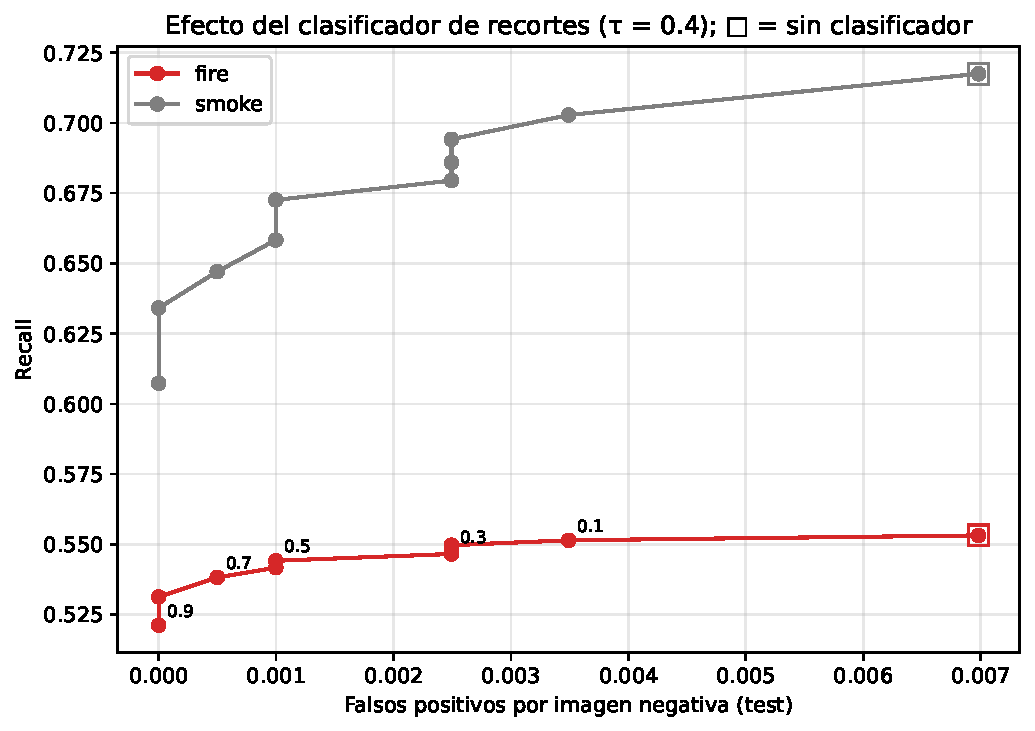
\includegraphics[width=0.82\columnwidth]{clasificador_recall_vs_fp}
\caption{H4: recall por clase contra falsos positivos por imagen negativa de prueba al variar el umbral del clasificador (R1, $\tau=0{,}4$). El cuadrado marca el sistema sin clasificador.}
\label{fig:clf}
\end{figure}

\subsection{Sistema completo sobre video (H3)}

\begin{figure}[t]
\centering
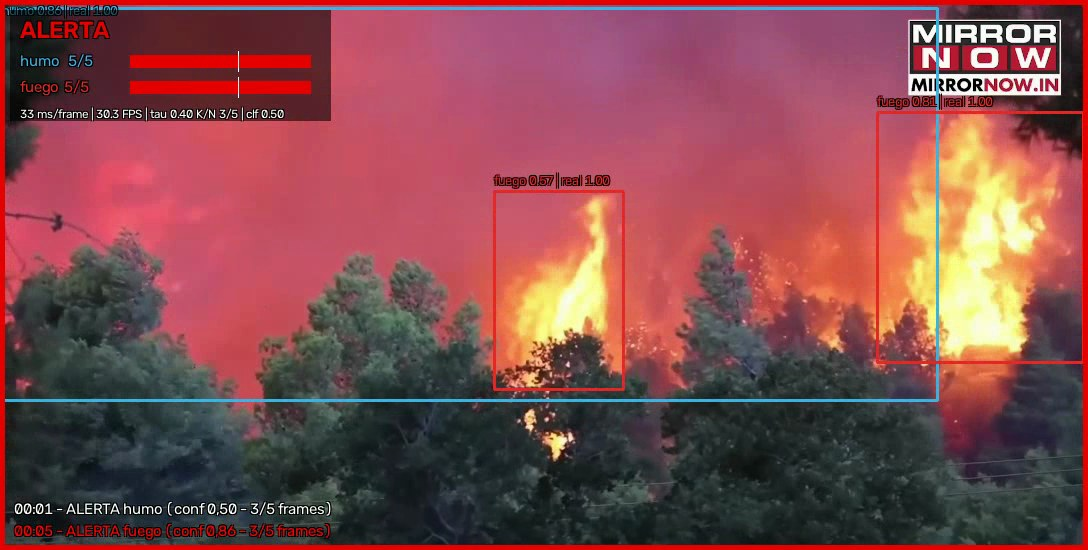
\includegraphics[width=\columnwidth]{demo_frame.jpg}
\caption{Demo del sistema sobre video: cajas de fuego (rojo) y humo (celeste) confirmadas por el clasificador, estado \textsc{alerta}, contador K/N por clase, latencia por frame y registro de eventos.}
\label{fig:demo}
\end{figure}

Procesamos dos clips de cobertura periodística de incendios forestales (\SI{60.5}{s} y \SI{41.5}{s}, \SI{50}{fps}) con el sistema completo (R1, clasificador, $\tau=0{,}4$, $K/N=3/5$). En ambos el sistema entra en alerta de humo en torno al primer segundo y de fuego antes de los \SI{7}{s}, y el detector más clasificador corre a 30--40 FPS en la CPU de una notebook.

El experimento dejó una observación de diseño: $N$ debe fijarse en tiempo y no en frames. Procesando todos los frames a \SI{50}{fps}, la ventana de 5 frames cubre \SI{0.1}{s}; el parpadeo natural de las detecciones vacía el buffer y el mismo incendio dispara una alerta nueva cada pocos segundos (49 eventos en los dos clips). Procesando uno de cada diez frames (\SI{5}{fps}, ventana de \SI{1}{s}) los eventos bajan a 12, y en el segundo clip, una única escena continua, a uno por clase. El primer clip es un montaje de varias escenas, por lo que parte de sus eventos corresponde a cortes de edición.

% TODO (si llegan): reemplazar este párrafo por el barrido de barrido_alerta.ipynb
% (falsas alarmas/hora vs. latencia de alerta para tau y K/N, con y sin clasificador)
% sobre clips de cámaras fijas con t_evento anotado y un clip sin evento.
Estos clips no permiten medir la latencia de alerta ni las falsas alarmas por hora, porque el incendio ya es visible desde el primer frame y no incluyen tramos sin evento. Por eso H3 queda evaluada solo de forma cualitativa.

\subsection{Análisis de errores}

% \begin{figure*}[t]
% \centering
% 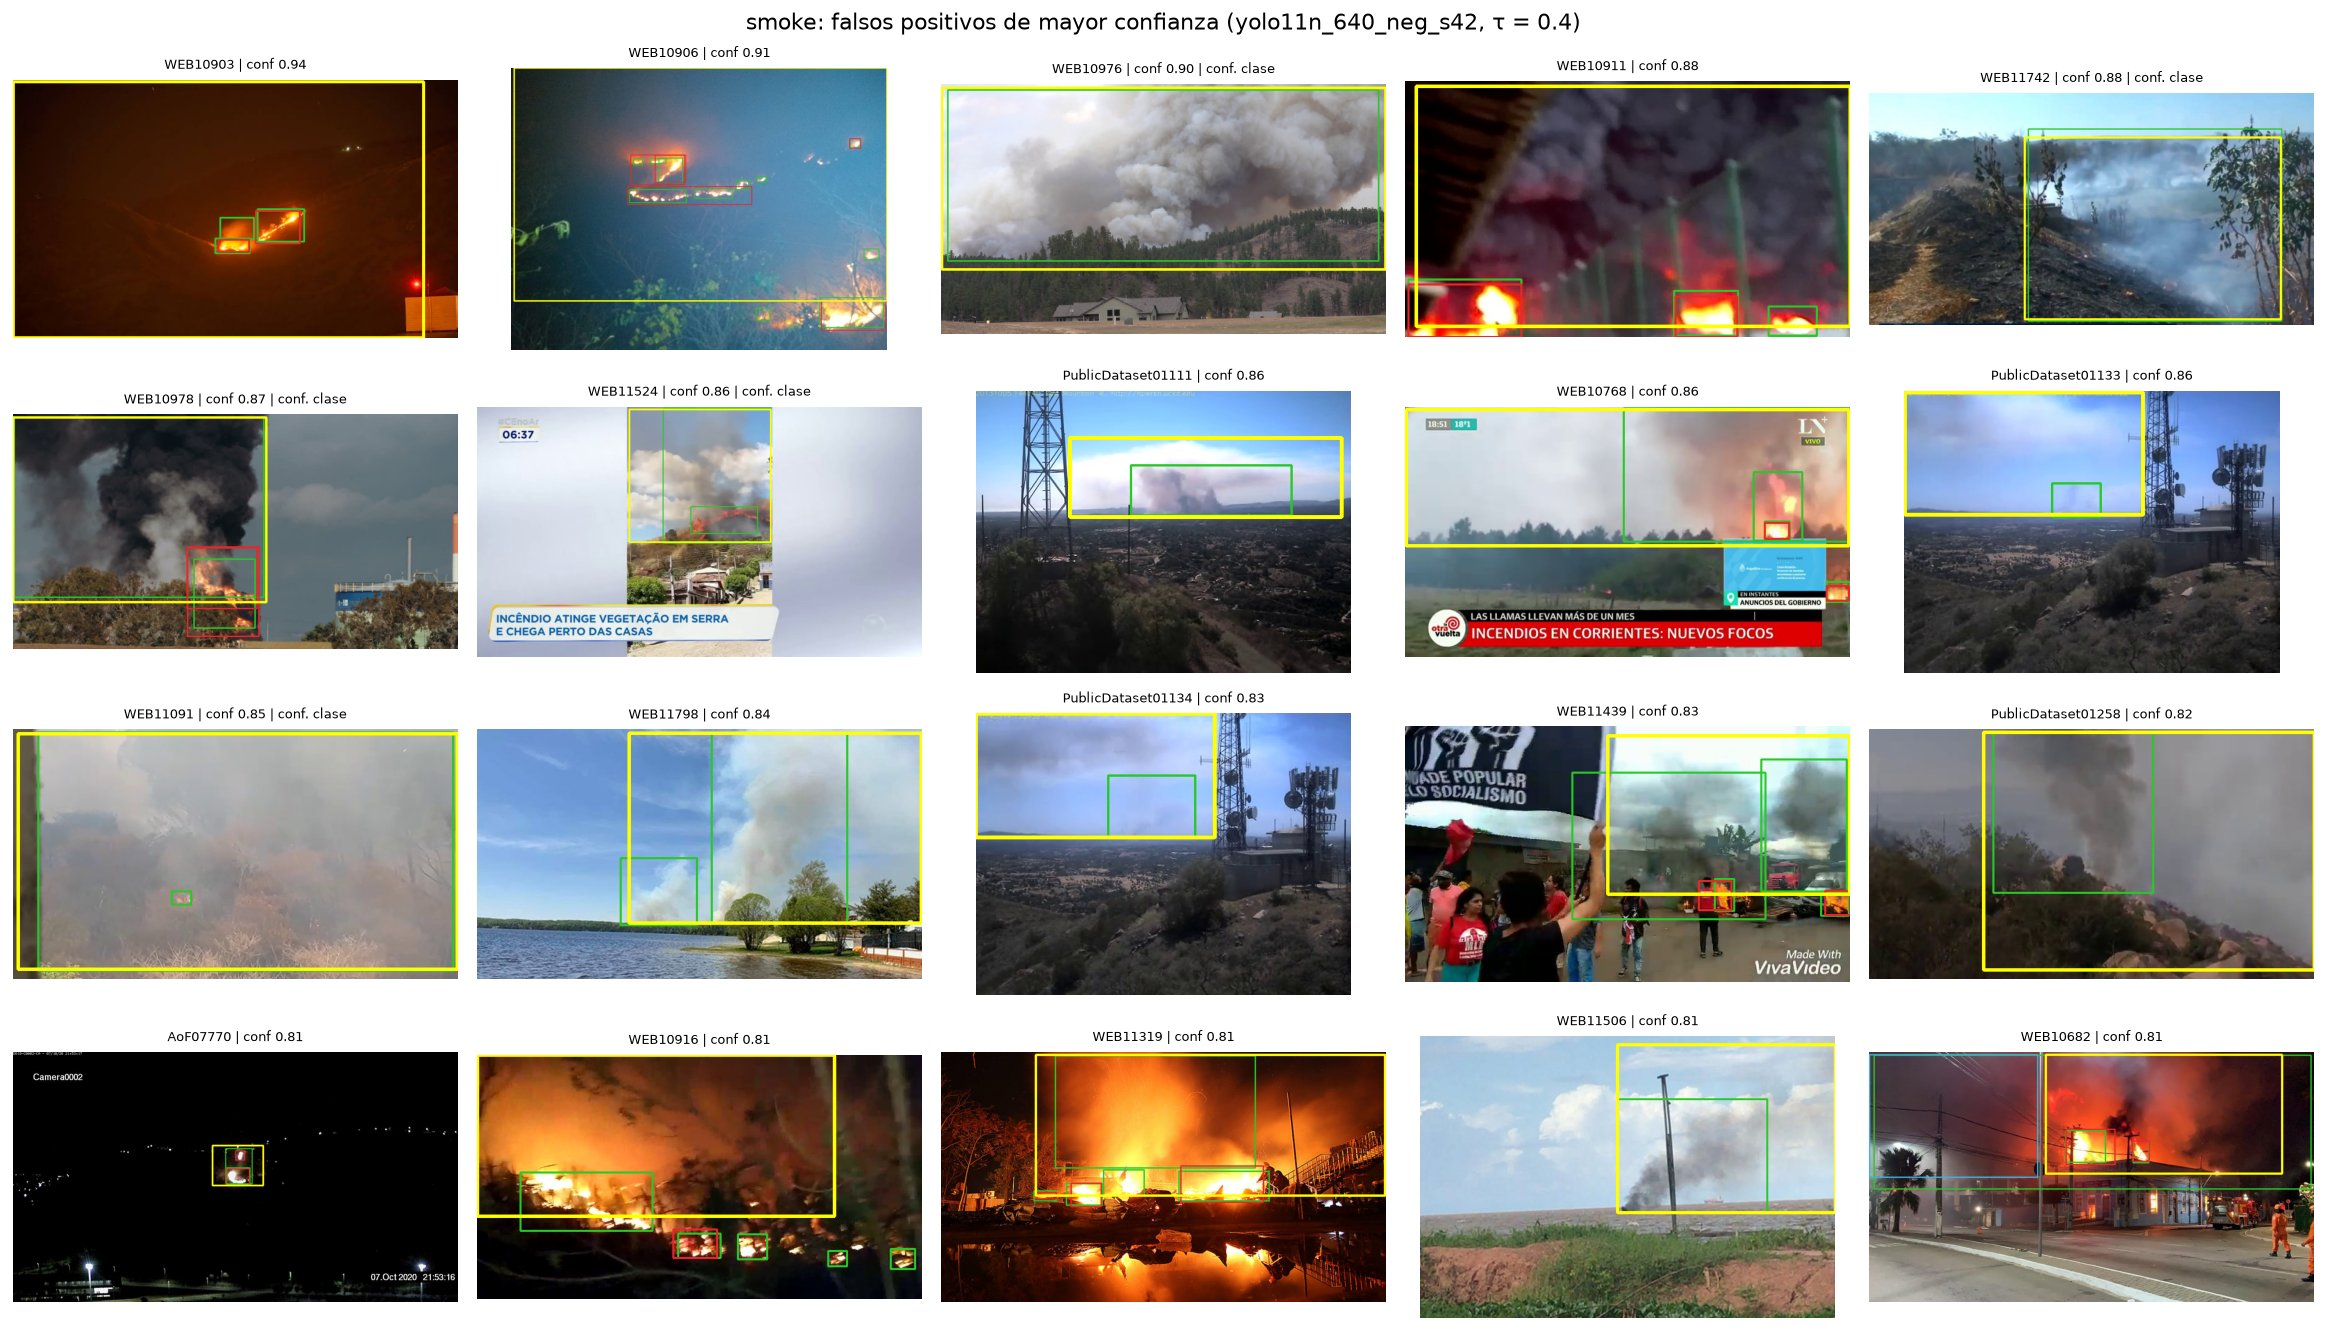
\includegraphics[width=\textwidth]{errores_fp_humo.jpg}
% \caption{Los 20 falsos positivos de humo de mayor confianza de R1 ($\tau=0{,}4$). En amarillo, la predicción contada como falso positivo; en verde, el \textit{ground truth}; en rojo y celeste, otras predicciones de fuego y humo. En muchos casos hay humo visible dentro de la caja y la discrepancia es de granularidad de la anotación.}
% \label{fig:errores}
% \end{figure*}

Revisamos los 20 falsos positivos de mayor confianza y los 20 falsos negativos de mayor área por clase de R1 a $\tau=0{,}4$. Ninguno de esos falsos positivos cae en una imagen negativa, y 5 son confusiones entre clases (humo detectado como fuego o al revés). En humo, una parte importante de los falsos positivos de alta confianza son predicciones correctas penalizadas por la anotación: el modelo marca toda la columna de humo mientras que el \textit{ground truth} la divide en cajas más chicas o cubre solo una parte, de modo que el IoU queda por debajo de \num{0.5} (Fig.~\ref{fig:errores}). Esto sugiere que las métricas de humo subestiman la utilidad del detector para la tarea de alerta, donde lo que importa es la presencia y no el contorno exacto.
% TODO: completar results/errores_causas.csv y agregar aquí la distribución de causas.

% ---------------------------------------------------------------------------
\section{Conclusiones}

\begin{enumerate}
\item \textbf{Las imágenes negativas son la decisión de datos más importante.} Incluirlas en el entrenamiento reduce 44 veces la fracción de imágenes sin incendio con falsos positivos (\SI{28.8}{\percent} a \SI{0.65}{\percent}) sin pérdida de recall.
\item \textbf{Para CPU, el modelo \textit{nano} es el punto de equilibrio.} El modelo \textit{medium} mejora el mAP50 en solo \num{0.020} con 5,3 veces más latencia; \textit{nano} permite procesar 18 FPS en CPU.
\item \textbf{La resolución ayuda poco con el fuego incipiente.} Pasar a \SI{960}{px} mejora 3,4 puntos el recall de fuego chico a 1,65 veces el costo, y el recall de esa categoría sigue por debajo de \num{0.45}: es el principal cuello de botella del sistema.
\item \textbf{El clasificador de recortes es un filtro barato y ajustable.} Con un \SI{12}{\percent} de latencia adicional reduce siete veces los falsos positivos en negativas, a cambio de 4,5 puntos de recall en humo; su umbral es un parámetro operativo.
\item \textbf{El criterio temporal debe parametrizarse en segundos.} Una ventana definida en frames depende de la tasa de cuadros: a \SI{50}{fps} no filtra nada, mientras que a \SI{5}{fps} los eventos de alerta se reducen cuatro veces.
\item \textbf{El test oficial de D-Fire es optimista.} Cerca de la mitad de sus imágenes tienen un casi-duplicado en entrenamiento; recomendamos separar por cámara o escena al evaluar generalización.
\item \textbf{El mAP de humo subestima la utilidad para alerta.} Muchos falsos positivos de alta confianza son discrepancias de granularidad con la anotación, no errores de presencia.
\end{enumerate}

\textbf{Limitaciones y trabajo futuro.} Todos los detectores se entrenaron con una sola semilla, por lo que diferencias menores a \num{0.01} de mAP no son concluyentes. La evaluación en video es cualitativa y usa clips periodísticos, no cámaras fijas de vigilancia. Queda pendiente medir falsas alarmas por hora y latencia de alerta sobre secuencias de cámaras fijas con el inicio del evento anotado, como las de FIgLib \cite{dewangan2022figlib}, y evaluar el clasificador sobre un conjunto de estrés externo con nubes, niebla, atardeceres, luces nocturnas y reflejos.
% TODO: si se arma el set de estrés (analisis_errores.ipynb, sección 7), agregar sus resultados.

El código, los pesos entrenados y las instrucciones de reproducción están disponibles en \url{https://github.com/AndreTati/deteccion_incendios}.

\twocolumn[{%
  \centering
  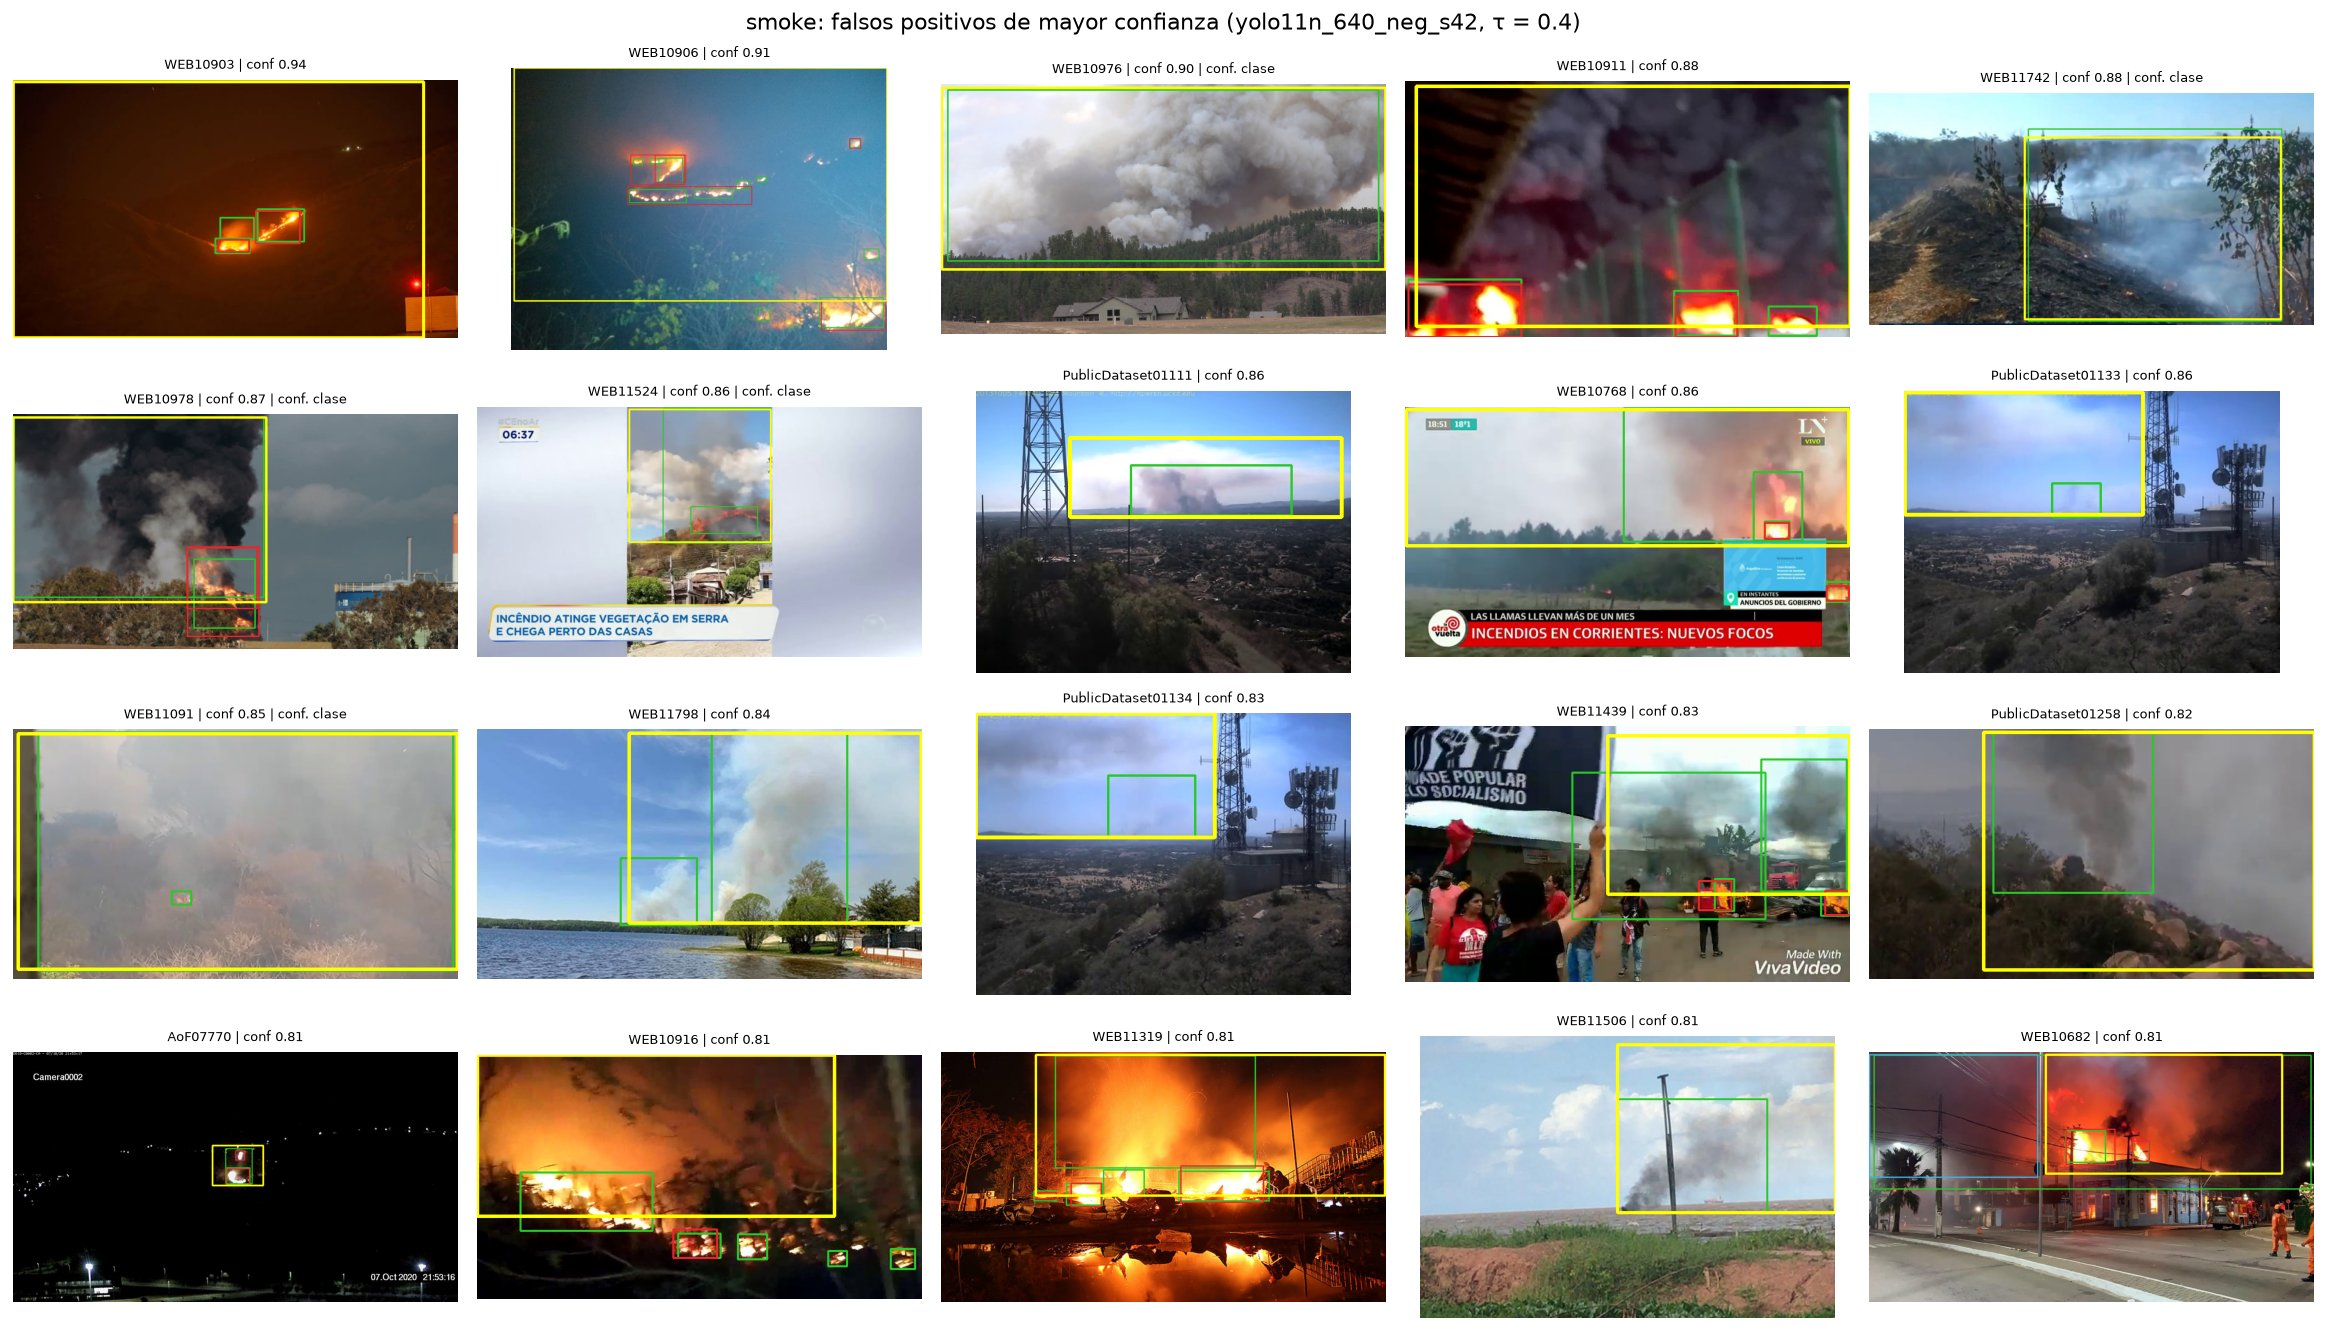
\includegraphics[width=\textwidth]{errores_fp_humo.jpg}
  \captionof{figure}{Los 20 falsos positivos de humo de mayor confianza de R1 ($\tau=0{,}4$). En amarillo, la predicción contada como falso positivo; en verde, el \textit{ground truth}; en rojo y celeste, otras predicciones de fuego y humo. En muchos casos hay humo visible dentro de la caja y la discrepancia es de granularidad de la anotación.}
  \label{fig:errores}
  \vspace{1.5em}
}]

\bibliographystyle{IEEEtran}
\bibliography{refs}

\end{document}
